%--------Arquitectura y Diseño de componente para RBox
%--------Daniel Ochoa John
%--------20/07/2014
\newcolumntype{L}[1]{>{\raggedright\let\newline\\\arraybackslash\hspace{0pt}}m{#1}}
\newcolumntype{C}[1]{>{\centering\let\newline\\\arraybackslash\hspace{0pt}}m{#1}}
\newcolumntype{R}[1]{>{\raggedleft\let\newline\\\arraybackslash\hspace{0pt}}m{#1}}

\chapter{Arquitectura y Diseño de componente para RBox}
\label{cap:arquitectura}

En este capítulo se tratará la arquitectura y diseño de un componente para RBox que permitirá comunicarse apropiadamente con el componente de detección de comunidades ya descrito en el Capítulo 3. En primer lugar, se realizará una descripción de la arquitectura del componente, incluyendo su inclusión en RBox. Luego, se mostrará el diseño de clases con los componentes que ha sido necesario construir y se describen las razones de inclusión de cada uno de ellos. Posteriormente, se tratan los impactos que este componente ha tenido sobre las distintas capas de  RBox. Finalmente, se detalla la comunicación entre componentes y como se detona la detección de comunidades al recomendar.

\section{Descripción Arquitectural}

En esta sección se describe, en líneas generales, la arquitectura de RBox y su integración con las nuevas piezas de \textit{software} que permitirán consumir el servicio de detección de comunidades descrito anteriormente. La Figura \ref{fig:arq-im1} muestra los componentes utilizados y sobre los cuáles se ha diseñado.

\begin{figure}
  \centering
  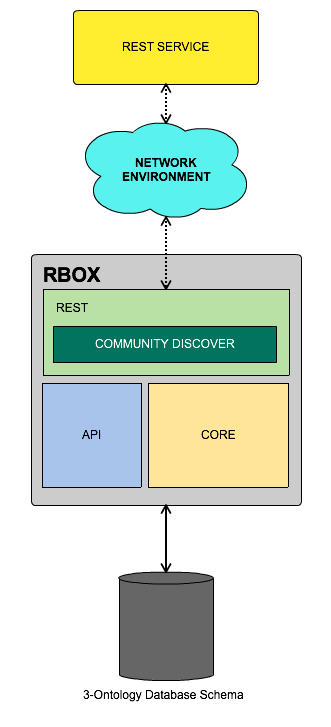
\includegraphics[scale=.6]{images/Figura4-1}
  \caption{\em Diagrama que representa la arquitectura formada por los componentes de RBox.}
  \label{fig:arq-im1}
\end{figure}


En primer lugar, se requiere de un mecanismo de persistencia para la información requerida y generada por el sistema:

\begin{itemize}
  \item \textbf{3-Ontology \textit{Database Schema}:} es un esquema relacional basado en el modelo conceptual de la 3-Ontology. Su función es persistir y proveer información, desde y hacia RBox, respecto de los distintos eventos que ocurran en la(s) red(es) social(es) que se estén monitoreando, con el objetivo final de generar una recomendación.
\end{itemize}

El siguiente componente es RBox, que se compone de distintos submódulos. Originalmente y, antes de este trabajo de Tesis, solamente existían dos submódulos:

\begin{itemize}
  \item \textbf{API:} es un conjunto de interfaces que definen las propiedades estándar de todos los objetos que quieran extender, utilizar las propiedades de RBox o construir recomendadores. En este submódulo también se incluye la definición de las interfaces que representan a los contenedores de sentido y la lógica de la 3-Ontology.
  \item \textbf{CORE:} una implementación del API basada en distintos componentes. En este submódulo se implementa la capa \textit{Data Access Object} (DAO) a través de componentes que utilizan JDBC. Además, se incluyen implementaciones base para distintos tipos de eventos y recomendadores.
\end{itemize}

Luego de finalizado este trabajo de Tesis, se han agregado otros módulos a RBox, que tiene que ver con el manejo de servicios REST.

\begin{itemize}
  \item \textbf{REST:} un submódulo de RBox que permite realizar \textit{request} de tipo REST a distintos servicios. En particular, se ha incluído un submódulo llamado \textit{Community Discover}, que es una implementación de un cliente REST para comunicarse con el servicio de detección de comunidades.
  \item \textbf{\textit{Community Discover}:} un submódulo que se preocupa de proveer desde y hacia RBox un mecanismo de consumo, procesamiento y encapsulación de la información necesaria para el manejo de las comunidades detectadas por el servicio de detección de comunidades. La persistencia de las comunidades detectadas se realiza a través de la capa DAO, que existe en el \textit{core} de RBox.
\end{itemize}

Como se puede apreciar en la Figura \ref{fig:arq-im1}, es el componente REST de RBox el que se comunica, a través de un \textit{Network Environment} acorde a la realidad de la aplicación, con un servicio REST y, en este caso en particular, la comunicación se realiza con el servicio de detección de comunidades.  Ahora, es necesario describir con un mayor detalle el componente \textit{Community Discover}, y las piezas que se han creado para su integración con RBox.

\section{Diseño de Clases}

En esta sección se describe detalladamente el componente \textit{Community Discover} mencionado en la arquitectura. Primero cada uno los submódulos definidos y luego, para cada uno de ellos, una descripción clase a clase.

La Figura \ref{fig:arq-im2} muestra un diagrama con la comunicación entre los componentes de \textit{Community Discover}. Se ha incluído el Core de RBox para ilustrar que el recién mencionado:

\begin{enumerate}[I]
  \item Solo se ve impactado por la respuesta del servicio de \textit{Community Discover}.
  \item Puede consumir únicamente una capa de métodos utilitarios de conversión de datos llamada Converter.
\end{enumerate}

\subsection{Model}

Este componente define un \textit{Data Transfer Object} (DTO), el cual es un modelo que será utilizado en los proceso que involucren al servicio REST.  La Tabla \ref{tab:arq-tab01} muestra las clases que contiene este componente:

\begin{table}[H]
  \begin{center}
    \caption{Clases involucradas en la composición de \textit{Model}.}
    \label{tab:arq-tab01}
      \begin{tabular}{|L{4cm}|L{10cm}|}
        \hline
        \textbf{Clase} & \textbf{Descripción}\\ \hline
         \textit{CommunityModel} & Clase que define un modelo de comunidad, a partir de un arreglo de \textit{NodeModel}.\\ \hline
         \textit{EdgeModel} & Clase que define un modelo de arista  (en inglés, \textit{edge}), a partir de un origen y un destino, representados por un ID de tipo Long. \\ \hline
         \textit{NodeModel} & Clase que define un modelo para un nodo (en inglés, \textit{node}), a partir de un ID de tipo Long y un String representativo como nombre. \\ \hline
      \end{tabular}
  \end{center}
\end{table}

\subsection{Wrapper}

Este componente provee un medio de encapsulación de los datos que se envían desde y hacia el servicio Web. Puede ser descrito como un contenedor de información que se envía o recibe dependiendo de si es un \textit{request} al servicio o un \textit{response} del servicio. La Tabla \ref{tab:arq-tab02} muestra las clases que contiene este componente:

\begin{table}[H]
  \begin{center}
    \caption{Clases involucradas en la composición de \textit{Wrapper}.}
    \label{tab:arq-tab02}
      \begin{tabular}{|L{4cm}|L{10cm}|}
        \hline
        \textbf{Clase} & \textbf{Descripción}\\ \hline
         \textit{CommunityWrapper} & Esta clase define un contenedor de comunidades a partir de un arreglo de objetos \textit{CommunityModel}. Es como se traduce la respuesta del servicio de detección de comunidades.\\ \hline
         \textit{\textit{Graph}Wrapper} & Esta clase define un contenedor de grafo a partir de una lista de elementos \textit{EdgeModel} y una lista de elementos \textit{NodeModel}. Es como se envía la solicitud al servicio de detección de comunidades. \\ \hline
      \end{tabular}
  \end{center}
\end{table}

\subsection{\textit{Client}}

Este componente consiste en una clase cuyo propósito es realizar el \textit{request} correspondiente al servicio REST, a partir de un grafo encapsulado de tipo \textit{\textit{Graph}Wrapper} y también de persistir los resultados del \textit{response} a través del uso de \textit{\textit{CommunityDAO}} existente en el CORE de RBox. La Tabla \ref{tab:arq-tab03} muestra las clases de este componente:

\begin{table}[H]
  \begin{center}
    \caption{Clases involucradas en la composición de \textit{\textit{Client}}.}
    \label{tab:arq-tab03}
      \begin{tabular}{|L{4cm}|L{10cm}|}
        \hline
        \textbf{Clase} & \textbf{Descripción}\\ \hline
         \textit{Community Discover}\textit{Client} & Esta clase define a un cliente que permite conectarse y consumir el servicio de detección de comunidades, dado un \textit{\textit{Graph}Wrapper} como \textit{request}, recibe un \textit{CommunityWrapper} como \textit{response}.\\ \hline
         \textit{\textit{Graph}Wrapper} & Esta clase define una versión particular para un cliente del servicio de detección de comunidades, ya que permite obtener y recrear el ejemplo de uso de los algoritmos de los endpoints del servicio, de tal forma como se mostró en el Capítulo \ref{cap:servicio}. Al ser solo servicios GET, solo envía una solicitud a una URL en el \textit{request}. El \textit{response} del servicio es un objeto \textit{CommunityWrapper}. \\ \hline
      \end{tabular}
  \end{center}
\end{table}

\subsection{Service}

Este componente consiste en una especialización de los servicios de la 3-Ontology. En este caso en particular, como \textit{Portrait} (del español Retrato, ver Capítulo 2) es el servicio de la 3-Ontology que tiene que ver con las comunidades, se provee una especialización de el. La especialización del servicio también tiene que ver con adoptar una estrategia inteligente de persistencia en dos niveles. Este mecanismo ha sido denominado \textit{community cache}. Lo anterior se resume en la Tabla \ref{tab:arq-tab04}.

El mecanismo de \textit{community cache}, en un primer nivel, permite controlar si la detección y persistencia se realiza solamente cuando el usuario (al que se quiere otorgar una recomendación) no tiene comunidades asociadas en el modelo de la 3-Ontology. En el segundo nivel, tiene que ver si para la persistencia se toma en cuenta el hecho de que la comunidad ya forma parte del modelo de la 3-Ontology, considerando el conjunto de usuarios que la forman.

\begin{table}[H]
  \begin{center}
    \caption{Clases involucradas en la composición de \textit{Service}.}
    \label{tab:arq-tab04}
      \begin{tabular}{|L{4cm}|L{10cm}|}
        \hline
        \textbf{Clase} & \textbf{Descripción}\\ \hline
         CommunityExtension\textit{Portrait} & Esta clase hereda de Generic\textit{Portrait} que existe en el Core de RBox y resume un servicio que permite detectar y persistir comunidades para un usuario, de manera forzada o bien, cuando no existen explícitamente en el esquema relacional de datos. El manejo de una estrategia de \textit{community cache} para persistir comunidades también está definido en este servicio.\\ \hline
      \end{tabular}
  \end{center}
\end{table}

\subsection{Converter}

Este componente permite realizar transformaciones desde un tipo de dato a otro. Es utilizado en \textit{Community Discover} para transformar una serie de \textit{Event}os del esquema de 3-Ontology a un \textit{\textit{Graph}Wrapper}, que es el formato aceptado por el servicio de detección de comunidades. Además, permite realizar otro tipo de transformaciones, como por ejemplo, transformar un \textit{\textit{Graph}Wrapper} en un objeto \textit{Graph} para visualizar su estructura y conexiones, tal como se realizó en el ejercicio del Club de Karate de Zachary. La Tabla \ref{tab:arq-tab05} describe las clases que forman esta pieza.

\begin{table}[H]
  \begin{center}
    \caption{Clases involucradas en la composición de \textit{Converter}.}
    \label{tab:arq-tab05}
      \begin{tabular}{|L{4cm}|L{10cm}|}
        \hline
        \textbf{Clase} & \textbf{Descripción}\\ \hline
         \textit{\textit{Event}WrapperConverter} & Esta clase utiliza el patrón Generics de JAVA para logar, dado una clase que herede de \textit{Event} y una clase que herede de \textit{Item}Dao, convertir instancias de \textit{Event} en un \textit{GraphWrapper} con tal de ser enviado al servicio de detección de comunidades.\\ \hline
         \textit{GraphWrapperConverter} & Esta clase se encarga de realizar una transformación de un objeto \textit{GraphWrapper} en un objeto \textit{Graph} específico de una API llamada \textit{GraphStream}\footnote{Es una librería para JAVA, que permite el manejo de grafos dinámicos. Sitio oficial en http://graphstream-project.org/}. Esto permite, entre otras cosas, renderizar y visualizar el grafo resultante del proceso de \textit{Wrapping}.\\ \hline
      \end{tabular}
  \end{center}
\end{table}

Ya con los componentes descritos, es necesario analizar el impacto que esto tiene en el modelo actual de RBox, repasando capa a capa las modificaciones que han sido necesarias para dar soporte, sobre todo, a la persistencia de datos en un esquema relacional.

\begin{figure}
  \centering
  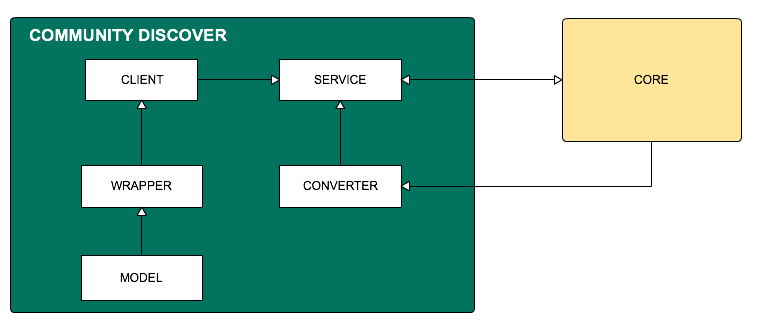
\includegraphics[scale=.6]{images/Figura4-2}
  \caption{\em Diagrama con la comunicación entre los componentes de \textit{Community Discover}}
  \label{fig:arq-im2}
\end{figure}

\section{Impacto en el modelo actual}

En esta sección se resumen los cambios que se han realizado en el Core de RBox para permitir el funcionamiento del ciclo de detección y persistencia de comunidades.

\subsection{\textit{Event}os}

Se han añadido dos tipos de eventos a RBox: \textit{mentioning} y \textit{replying}, como representación del modelo de interacciones que provee Twitter. No obstante, la implementación es genérica y son reutilizables en otra red social que utilice este tipo de eventos. Por ende, ambos son necesarios para contextualizar la herramienta a la red social que se analizará en el capítulo siguiente y poseen un valor de tipo String. Se han añadido versiones mutables e inmutables de ambos eventos.

\subsection{DAO}

Se han implementado la interfaz \textit{CommunityDAO} para el manejo de comunidades con esquemas relacionales a través de JDBC. Además, RBox no tenía implementado un mecanismo de persistencia en esquemas relacionales y solamente estaba enfocado en consumir información de este medio. Por lo tanto, para poder persistir las comunidades detectadas, ha sido necesario añadir esta funcionalidad y preparar \textit{statements} que faciliten el proceso de insertar comunidades y asociar usuarios a las comunidades a las que pertenecen. Se ha creado un DAO que facilite el acceso a los \textit{Item}s, ya que son parte fundamental de la generación de los \textit{\textit{Graph}Wrapper}.

\subsection{Extensions}

Se ha creado un nuevo módulo en RBox, que tiene que ver con el manejo de extensiones de funcionalidades. El funcionamiento está basado en transformaciones y encapsulamientos de datos, por lo que toda extensión, detección de comunidades incluída, debe definir sus propios servicios de transformación, que hereden de la interfaz Wrapper, desde y hacia 3-Ontology del esquema de datos en particular que cada extensión maneje (texto plano, xml, json, abstracto mediante objetos, entre otros).

En el caso particular de la extensión de detección de comunidades, se ha definido la interfaz \textit{CommunityExtension}, que utiliza, mediante \textit{Generics}, dos clases que heredan de la interfaz Wrapper para definir los servicios que esta extensión provee. En el segmento de código que muestra la Figura \ref{fig:arq-im3} está la definición de esta interfaz. En \textit{Community Discover}, la clase \textit{Community Discover}\textit{Client} es la que implementa esta interfaz, ya que es la que provee el servicio de detección y persistencia de comunidades.

\begin{figure}[H]
  \centering
  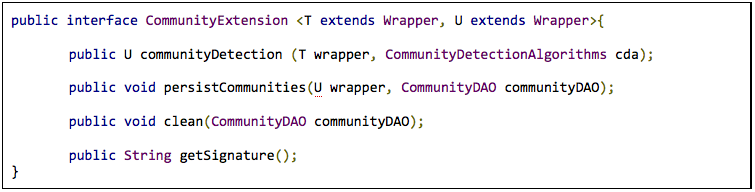
\includegraphics[scale=.6]{images/Figura4-3}
  \caption{\em Código que muestra la interfaz que debe implementar todo servicio de detección de comunidades.}
  \label{fig:arq-im3}
\end{figure}

Como se ha descrito, las modificaciones en el Core de RBox son menores y el mayor impacto y la lógica de los servicios y procesos reside en el componente \textit{Community Discover}. Luego, es hora de describir el proceso completo de comunicación entre los componentes mencionados en este capítulo.

\section{Comunicación entre componentes}

En esta sección se detalla el proceso de comunicación con todos los componentes ya descritos, a partir de un ejemplo de código que se muestra en la Figura \ref{fig:arq-im4}. En primer lugar, se obtiene una instancia de JDBCDAO y, con esta, se obtienen los eventos registrados en el medio persistente. Luego, se genera una instancia de GenericTrace utilizando como parámetro a los eventos obtenidos anteriormente. Posteriormente, se obtiene una lista de \textit{UserHistory}, agrupando los eventos para cada usuario.

\begin{figure}[H]
  \centering
  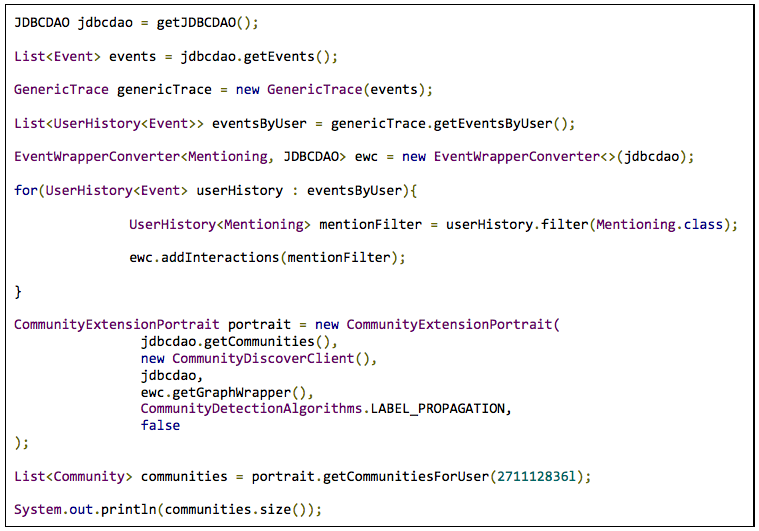
\includegraphics[scale=.6]{images/Figura4-4}
  \caption{\em Código que muestra la interacción entre los distintos componentes del servicio.}
  \label{fig:arq-im4}
\end{figure}


Una vez que se tiene el listado de \textit{User}History es necesario construir el encapsulador de eventos a un \textit{\textit{Graph}Wrapper}. Para esto se instancia un \textit{\textit{Event}WrapperConverter} utilizando como definición de Generics a la clase \textit{Mentioning}, y a JDBCDAO. Esto implica que los eventos que serán encapsulados son aquellos que sean de tipo \textit{Mentioning}.  Posteriormente, y para cada evento por usuario, se filtran los eventos para obtener sólo a aquellos que correspondan a \textit{Mentioning} y son esas interacciones las que se añaden al encapsulador. Cuando se tienen todos los eventos encapsulados, se crea el servicio \textit{Portrait} que provee \textit{Community Discover}. Para esto necesita:

\begin{enumerate}
  \item Todas las comunidades existentes en el sistema.
  \item Un cliente del servicio REST de detección de comunidades.
  \item Una instancia de JDBCDAO para permitir la persistencia de comunidades, según corresponda.
  \item Una instancia de \textit{\textit{Graph}Wrapper} que encapsule los eventos, que será enviado como \textit{request} al servicio de detección de comunidades.
  \item El algoritmo que se quiere que el servicio utilice al momento de detectar comunidades.
  \item Un valor booleano para determinar si se hace uso del primer nivel de \textit{community cache}. En otras palabras, si las comunidades se detectan siempre (\textit{true}) o solamente cuando no existan comunidades para un usuario (false).
\end{enumerate}

%TODO: CODIGO

Finalmente, se obtienen las comunidades para un usuario en particular. Si el usuario no tiene comunidades estas serán detectadas y se muestra la cantidad de comunidades a las que este usuario pertenece.

\section{Resumen}

En este capítulo se ha presentado el componente que se ha añadido a RBox para permitir la comunicación con el servicio de detección de comunidades presentado en el capítulo anterior. Además, se ha realizado una descripción componente a componente de cada uno de los submódulos de \textit{Community Discover}, el módulo REST que permite detectar comunidades en base a los eventos almacenados en lógica 3-Ontology. Luego, se ha analizado el impacto que la añadidura de este componente ha tenido sobre el \textit{core} de RBox ya desarrollado, identificando componentes restantes y añadiendo componentes nuevos para permitir el manejo de extensiones. Finalmente, se ha mostrado un ejemplo de integración de todos los componentes necesarios para realizar una detección de comunidades en base a un tipo de evento.
